% Created 2018-04-13 Fri 10:37
\documentclass[titlepage]{article}
\usepackage[utf8]{inputenc}
\usepackage[T1]{fontenc}
\usepackage{graphicx}
\usepackage{grffile}
\usepackage{longtable}
\usepackage{wrapfig}
\usepackage{rotating}
\usepackage[normalem]{ulem}
\usepackage{amsmath}
\usepackage{textcomp}
\usepackage{amssymb}
\usepackage{capt-of}
\usepackage{hyperref}
\usepackage{mathptmx}
\author{Xiong ChenYu \\
U1521516C \\
EEE \\
}
\date{Oct. 20, 2017 \\
}
\title{
\includegraphics[width=\textwidth]{img/NTU.png} \\
[1\baselineskip] Report \\
On \\
EE4483/IM4483 \\
Artificial Intelligence and Data Mining \\
Continuous Assessment \\
BY FP growth \\
[2\baselineskip]}
\hypersetup{
 pdfauthor={Xiong ChenYu \\
U1521516C \\
EEE \\
},
 pdftitle={
\includegraphics[width=\textwidth]{img/NTU.png} \\
[1\baselineskip] Report \\
On \\
EE4483/IM4483 \\
Artificial Intelligence and Data Mining \\
Continuous Assessment \\
BY FP growth \\
[2\baselineskip]},
 pdfkeywords={},
 pdfsubject={},
 pdfcreator={Emacs 27.0.50 (Org mode 9.1.9)},
 pdflang={English}}
\begin{document}

\maketitle
\tableofcontents

\listoftables
\listoffigures

\newpage

\section{Abstract}
\label{sec:org2a59890}
This report answer questions of the research and study on the continues assessment.
The algorithms used to do this project is the FP growth.

\begin{table}[htbp]
\caption{\label{tab:org748bca0}
System Specification}
\centering
\begin{tabular}{ll}
Usage & Application\\
\hline
System & Mac Sierra\\
Algorithm & FP growth\\
Language & Scala\\
Package & Spark\\
\end{tabular}
\end{table}

\newpage

\section{Question 1 (How many frequent itemsets have the minimum support of 20\%, 10\%, 5\%, and 3\% respectively?)}
\label{sec:orgf5e4b31}

\begin{table}[htbp]
\caption{\label{tab:org76e6c75}
Frequent itemsets counts}
\centering
\begin{tabular}{rr}
Minimum support (Unit : \%) & Itemsets size counts\\
\hline
20 & 20\\
10 & 68\\
5 & 268\\
3 & 659\\
\end{tabular}
\end{table}

\begin{center}
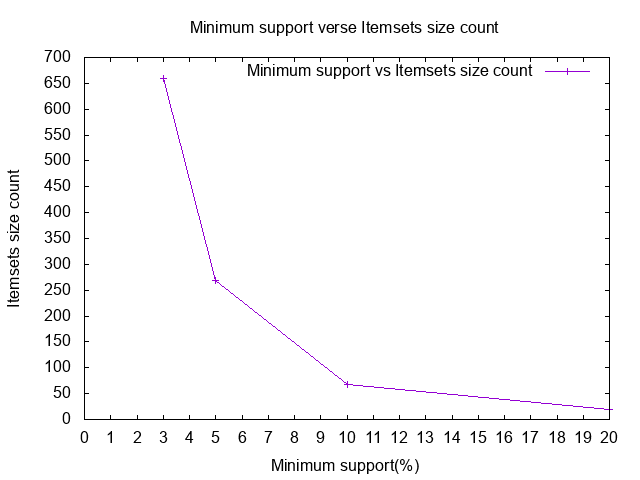
\includegraphics[width=.9\linewidth]{img/frequent.png}
\end{center}

\section{Question 2 (What are the respective percentages of frequent 3‐itemsets, and 2‐itemsets, with respect to all possible itemsets, which have a minimum support of 3\%?)}
\label{sec:org757358b}

\begin{table}[htbp]
\caption{\label{tab:org27cd88f}
3\% minsupport itemsets distribution}
\centering
\begin{tabular}{rr}
Itemsets size & Itemsets size count (Total: 659)\\
\hline
1 & 20\\
2 & 190\\
3 & 424\\
4 & 25\\
5 & 0\\
\end{tabular}
\end{table}

\begin{center}
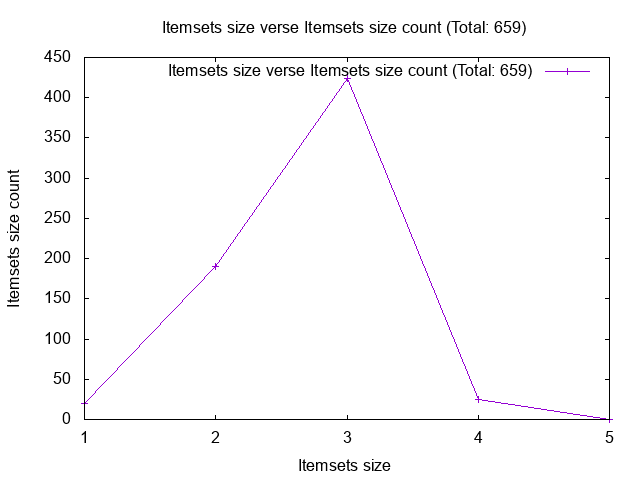
\includegraphics[width=.9\linewidth]{img/itemsets.png}
\end{center}

\begin{table}[htbp]
\caption{\label{tab:orgee0727c}
respective percentages}
\centering
\begin{tabular}{rl}
Itemsets size & Itemsets size count (Total: 659)\\
\hline
1 & \(\frac{20}{659} = 0.03\)\\
2 & \(\frac{190}{659} = 0.288\)\\
3 & \(\frac{424}{659} = 0.643\)\\
4 & \(\frac{25}{659} = 0.038\)\\
5 & \(\frac{0}{659} = 0\)\\
\end{tabular}
\end{table}
\section{Question 3 (How many association rules have a minimum confidence of 50\% and a minimum support of 5\% and 10\%, respectively? Briefly explain how the minimum support affects the strong rules generated. )}
\label{sec:org3f87eaf}

\begin{table}[htbp]
\caption{\label{tab:org9811961}
Rules counts on 50\% minimum confidence}
\centering
\begin{tabular}{rr}
Minimum Support(Unit: \%) & Rules counts\\
\hline
10 & 0\\
5 & 117\\
\end{tabular}
\end{table}

\section{Question 4 (List three association rules that have the highest support with 100\% confidence?)}
\label{sec:org96c0763}

\begin{table}[htbp]
\caption{\label{tab:org631ea84}
Rules(X itemsets => Y itemsets)}
\centering
\begin{tabular}{llr}
X itemsets & Y itemsets & support\\
\hline
Salad,Ham,Banana & Apple & 0.33\\
IceCream,Olive,Tea & Banana & 0.33\\
Ham,Coffee,Diaper & IceCream & 0.27\\
\end{tabular}
\end{table}

\section{Question 5 (Do you find any “interesting” rules? What are they? Briefly explain why.)}
\label{sec:orgb518588}


\addcontentsline{toc}{section}{References}

  \begin{thebibliography}{99}

  \bibitem{1}\textsc{En.wikipedia.org}\texttt{ (2017). Data Mining Algorithms In R/Frequent Pattern Mining/The FP-Growth Algorithm - Wikibooks, open books for an open world. [online] Available at: https://en.wikibooks.org/wiki/Data_Mining_Algorithms_In_R/Frequent_Pattern_Mining/The_FP-Growth_Algorithm [Accessed 7 Nov. 2017].}

  \bibitem{2}\textsc{En.wikipedia.org}\texttt{ (2017). Data Mining Algorithms In R/Frequent Pattern Mining/The FP-Growth Algorithm - Wikibooks, open books for an open world. [online] Available at: https://en.wikibooks.org/wiki/Data_Mining_Algorithms_In_R/Frequent_Pattern_Mining/The_FP-Growth_Algorithm [Accessed 7 Nov. 2017].}


\end{thebibliography}

\section{APPENDIX A}
\label{sec:org7170524}
\begin{verbatim}
package example
import org.apache.spark.{SparkContext, SparkConf}
import org.apache.spark.rdd.RDD
import org.apache.spark.mllib.fpm.FPGrowth

object Hello extends Greeting with App {

  println(greeting)
  val conf = new SparkConf().setAppName("Ex1_SimpleRDD").setMaster("local[4]")
  val sc = new SparkContext(conf)

  sc.setLogLevel("ERROR")

  val data = sc.textFile("data.csv")
  val transactions: RDD[Array[String]] = data.map(s => s.trim.split(", "))

  val fpg = new FPGrowth().setMinSupport(0.0276).setNumPartitions(10)
  val model = fpg.run(transactions)

  model.freqItemsets.collect().foreach { itemset =>
    println(itemset.items.mkString("[", ",", "]")
              + ", "
              + itemset.freq) }

  val minConfidence = 1
  model.generateAssociationRules(minConfidence).collect().foreach { rule =>
    println(rule.antecedent.mkString("[", ",", "]")
              + " => "
              + rule.consequent .mkString("[", ",", "]")
              + ", "
              + rule.confidence) }
  println(model.generateAssociationRules(minConfidence).collect().size)
  sc.stop()
}

trait Greeting {
  lazy val greeting: String = "hello"
}
\end{verbatim}
\end{document}